\section{La mise en place d'un cache pour les zones peuplées}
\subsection{Introduction}
Comme nous avons pu le voir dans la partie~\ref{introSolutions}, la mise en place d'un cache pour les zones peuplées permettrait d'améliorer la réactivité dans l'état (\textbf{W}). L'avantage de cette solution, même si l'issue n'était pas certaine, était de s'intéresser à une partie qui n'avait pas encore été étudié dans Blue Banana. Nous avons donc insérer un cache pour chaque nœud de l'environnement, celui-ci va fonctionner dans la continuité de liste des voisins d'un nœud. Nous expliquerons comment nous avons insérer le cache dans le code existant, les différents stratégies que nous avons pu mettre en place et les différents paramètres qui vont influencer le fonctionnent du cache. Nous avons aussi permis l'utilisation du cache pour aider ces nœuds voisins quand ceux-ci cherchent des nœuds.
 
\subsection{Explications de la mise en place du cache}

\subsubsection{Le fonctionnement global et la mise en place du cache dans Blue Banana}
Le fonctionnement global du cache consiste à garder en mémoire un certains nombre de nœuds qui faisait partis de la liste des voisins. Ainsi comme les mouvements de l'avatar sont désordonnés, il est possible qu'il retourne vers des nœuds qu'il vient de quitter. 
\par Sur la figure~\ref{cacheW}, nous pouvons les principales étapes du fonctionnement du cache. Au départ le cache et la liste des voisins sont remplis de différents nœuds. A l'étape 2, le nœud courant (rouge) se déplace et trouve des nouveaux voisins, ceux-ci sont insérés à sa liste des voisins. Deux nœuds sont alors déplacés vers le cache, ce qui pousse deux nœuds hors du cache. A la dernière étape, le nœud courant revient vers une zone qu'il connait, nous détaillerons après le mécanisme de recherche dans le cache, et il trouve deux nœuds dans son cache qui pourraient lui servir pour reconstruire son voisinage. Deux nœuds du cache sont alors insérés dans la liste des voisins du nœud courant, ce qui envoie deux nœuds de cette liste vers le cache. Dans cette exemple, plusieurs nœuds peuvent se déplacer en même temps, ce qui est le cas dans une seul des solutions de cache mise en place.
	\begin{figure}[!h]
        \centering
        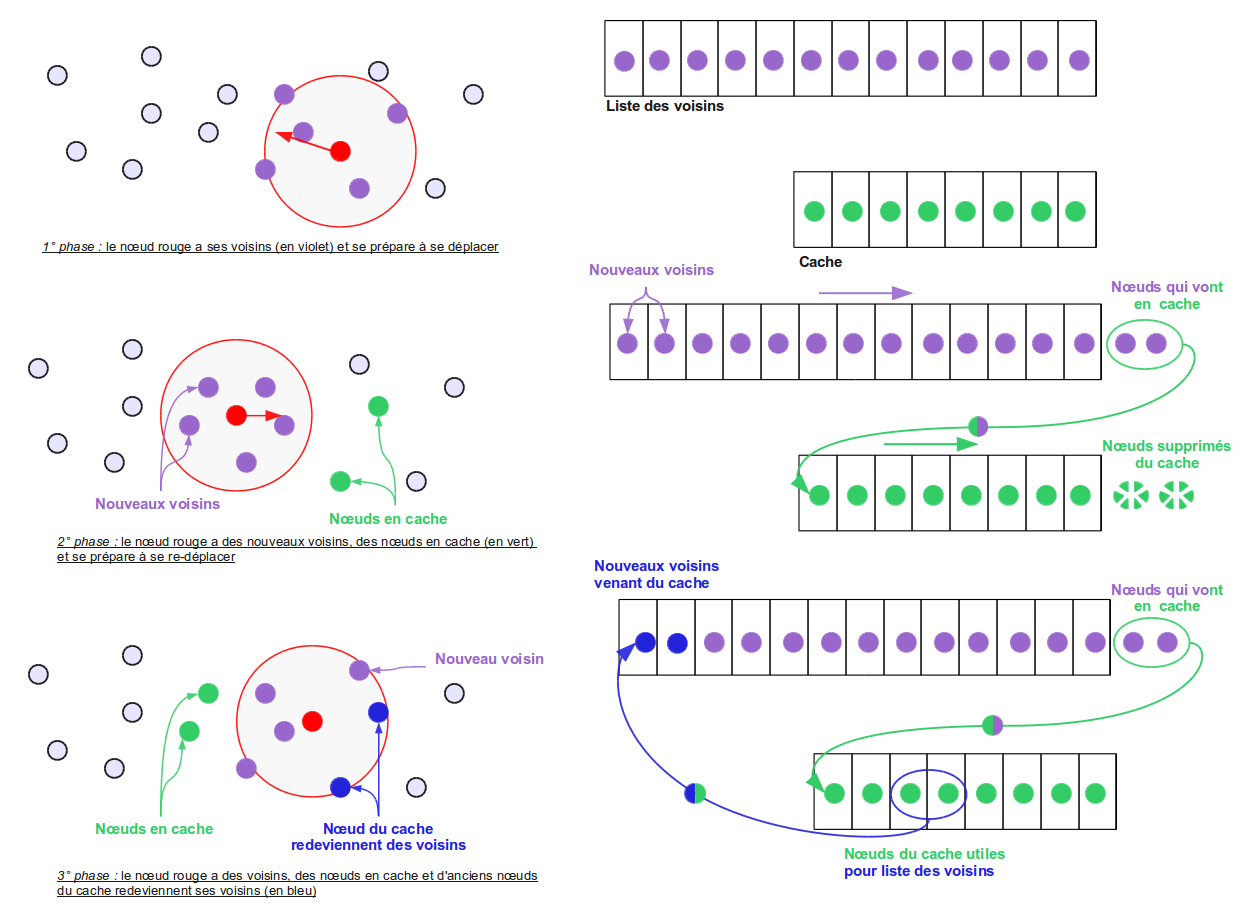
\includegraphics[scale=0.35]{./Ressources/Images/cacheWextends.png}
        \caption{Exemples du fonctionnement global du cache}
        \label{cacheW}
        \end{figure} 
\par Cette solution permet d'économiser des messages de découverte des voisins (SEARCH) dans le cas de changements de direction fréquents, il doit aussi nous permettre d'économiser des messages de connexions et déconnexion. Nous verrons dans la partie~\ref{resObsCache} les différents gains de la mise en place du cache, mais aussi les limites de celui-ci. Le cache est donc le prolongement de la liste des voisins pour nœud, mais contrairement à celui-ci , il n'est pas à jour, car un nœud est ajouté dans le cache avec les dernières informations que nous avions quand il était dans la liste des voisins. Nous avons donc mis en place un système de mis à jour du cache, pour avoir des informations le plus possible exact sur chaque nœud. Mais ce système va coûter cher en nombre de messages, et cela est encore plus vrai plus le cache est grand. Un mécanisme de datation des éléments du cache permet de savoir depuis quand date les informations de chacun. Ce mécanisme nous permet de contacté un nœud pour savoir s'il se trouve toujours à peu près au même endroit, et ainsi l'ajouter ou non à notre voisinage. Ces paramètres sont en options et nous verrons dans la partie~\ref{resObsCache} quelles sont les meilleures combinaisons d'options et si elles sont toutes utiles ou non.

\subsubsection{Les différentes versions du cache}

Deux versions, pour le fonctionnent du cache, ont été testé durant la phase d'implémentation. Nous parlons ici de la gestion des données dans la cache et non de la recherche dans celui-ci qui ce fera juste après. Au départ le cache était gérer selon le principe \textit{First In First Out}, la gestion du cache ne tenait pas compte des mises à jours, qui peuvent avoir lieu lors d'une requête vers un nœud du cache mais que celle-ci échoue car le nœud a trop bougé et qu'il a alors été mis à jour dans le cache. Une gestion du cache en fonction de la localité a aussi été mise en place, ce qui permet de faire sortir du cache les nœuds les plus éloignés de la position actuelle du nœud.
\par Deux implémentations ont aussi été testé pour la recherche dans le cache, l'une renvoie un résultat et l'autre renvoie plusieurs nœud à ajouter. Les tests \textbf{TODO}


\subsubsection{La modification du code existant pour insérer la recherche dans le cache}

 Avant de regarder les algorithmes de recherche dans le cache, nous allons vous expliquer comment ils sont appelé et quelles sont les modification introduites par rapport au code original. Lorsqu'un nœud rentre dans la fonction \textit{solipsisRecoverTopology} si le nœud est dans l'état \textbf{Wandering} alors on passe dans la fonction \textit{MaintainTopology}, sinon on effectue le traitement normal. Nous pouvons voir ci-dessous une partie du code de la fonction MaintainCache. Pour commencer, nous testons l'état de l'entité appelante, ensuite en fonction de la stratégie en fait un traitement particulier. Nous nous concentrerons sur la stratégie de base qui ajoute un seul nœud. La fonction de recherche nous renvoie donc un résultat. S'il n'est pas null et que sa date de mise à jour n'est pas trop ancienne, nous enlevons le nœud du cache, ajoutons le nœud à la liste des voisins et renvoyons 1 à la fonction appelante pour lui signifier que le traitement à été fait. Ensuite en fonction de la valeur de l'option \textit{contact\_node}, nous contactons ou non le nœud renvoyé par la fonction de recherche. Nous faisons ceci pour savoir s'il a beaucoup bougé depuis le dernier moment où nous l'avons vu. Nous retournons 0 pour signifier à la fonction appelante qu'aucun nœud n'a été ajouté et quelle peut faire le traitement de base.

\lstset{numbers=left,basicstyle=\scriptsize, numberstyle=\tiny, stepnumber=5, numbersep=5pt}

\lstinputlisting[title={Partie du code de la fonction MaintainCache},label={codeMaitainTopology}]{./Ressources/Documents/MaintainTopology.java}



\subsubsection{Les algorithmes de recherche dans le cache}
\par Nous allons expliquer comment nous recherchons les données dans le cache, et nous détaillerons les différentes pistes que nous avons testé dans un ordre chronologique. Tout d'abord nous avons sélectionner les nœuds en terme de distance, et de récupérer les plus proche de notre nouvelle position. Cette solution était assez simple à mettre en place, mais nous pensions que les résultats seraient meilleurs si nous prenions en compte la capacité à un nœud à aider à refaire l'enveloppe connexe du nœud courant. Nous avons alors implémenté une solution qui rendait un résultat positif si un nœud dans le cache permettait de reconstruire l'enveloppe du nœud (voir schéma~\ref{schemaEnvelopCache}). Cette solution a même été agrémenté d'un test si le nœud faisait avancé positivement l'enveloppe connexe mais ne la reconstruisait pas immédiatement.

	\begin{figure}[!h]
        \centering
        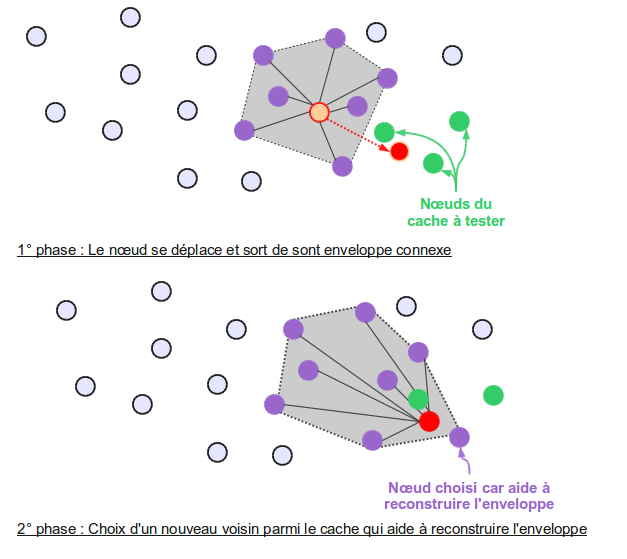
\includegraphics[scale=0.45]{./Ressources/Images/cacheReconstructEnvelop.png}
        \caption{Schéma montrant la solution de recherche dans le cache aidant à reconstruire l'enveloppe}
        \label{schemaEnvelopCache}
        \end{figure}
\par Le problème de cette solution est qu'elle privilégiait l'enveloppe connexe à la propriété de \textit{Local Awareness}. Car nous pouvons nous retrouver dans la situation, comme dans la figure~\ref{schemaEnvelopCache}, où un nœud ne fait pas parti de la liste des voisins alors qu'il se trouve dans l'enveloppe connexe. Cette solution nous donnez donc des résultats, pour les propriétés de Solipsis, qui était moins bon que la version sans le cache.  

\par Nous sommes alors revenu à une solution ressemblant à la première solution que nous avions mise en place. Chaque nœud comporte une zone de connaissance, nous avons donc décidé de nous servir de cette dernière pour réaliser les conditions dans la fonction de recherche. La fonction de recherche regarde donc si un nœud du cache est dans la zone de connaissance du nœud courant, si plusieurs correspondent un système pour choisir aléatoirement est mis en place, comme dans la recherche de voisin original.


\subsubsection{La mise en place de l'aide aux voisins grâce au cache}

Le cache d'un nœud va donc lui servir pour essayer de connaitre son environnement plus rapidement, mais il pourrait aussi aider les voisins du nœud. Dans cette optique, l'aide aux voisins a été mise en place. Ceci permet au cache d'avoir une autre utilisation, ce qui pourrait compenser la mise à jour si l'on souhaitais l'activer. Tout dépendra de la fréquence de mise à jour que l'on met et de l'efficacité ou non du cache. VOIR SI OK AVEC RESULTATS.
\par Lorsqu'un nœud cherche des voisins, il envoie un message SEARCH (voir schéma~\ref{schemaHelpCache}). Il suffit donc d'insérer une recherche dans le cache au bon endroit dans la fonction de traitement de ce message. Nous insérons donc, dans la fonction \textit{processSearchMsg}, une fonction de recherche dans le cache. Le nœud va tout d'abord regarder dans sa liste des voisins et si aucun ne correspond, nous regardons dans le cache si un nœud peut correspondre à la requête. La recherche dans le cache se fait, de façon similaire à une recherche dans le cache pour un nœud local, en utilisant la zone de connaissance que l'on aura préalablement transmis dans le message.

	\begin{figure}[!h]
        \centering
        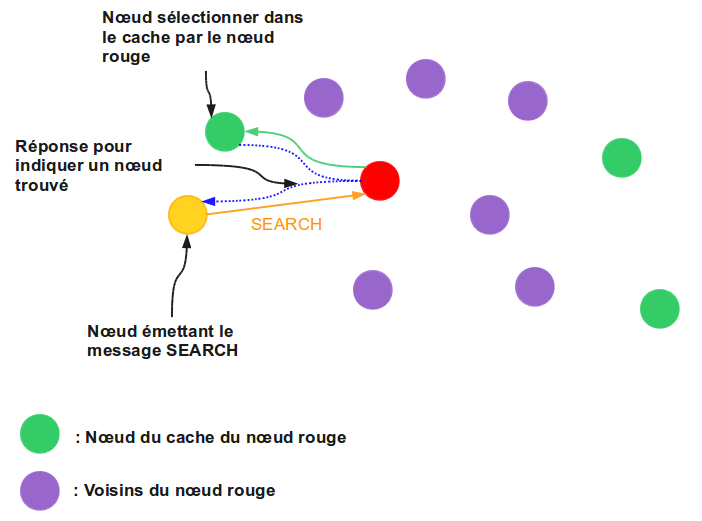
\includegraphics[scale=0.4]{./Ressources/Images/cacheHelp.png}
        \caption{Schéma montrant l'aide du cache pour le traitement d'un message SEARCH}
        \label{schemaHelpCache}
        \end{figure}

\subsection{Résultats et observations sur le cache}
\label{resObsCache}

Nous allons présenter les différents résultats sur le cache. Nous comparerons chaque version une de base où l'on ne trouve ni cache ni prefetch, et avec une version avec le prefetch implémenté dans Blue Banana.
Les principales métriques pour comparer les différents résultats sont la cohérence de la topologie et le nombre de message qui sont exprimées en fonction de la mobilité des avatars. Le calcul de la cohérence de la topologie consiste à mesurer, à chaque instant, le nombre de nœud qui sont dans la zone de connaissance d'un autre nœud mais qui ne fait pas parti des voisins de ce dernier.
TODO




\subsection{Conclusion et perspectives du cache} 



